% !TeX encoding = UTF-8
% !TeX program = pdflatex
% !TeX spellcheck = it_IT
\documentclass[binding=0.6cm]{sapthesis}
\usepackage{microtype}
\usepackage[italian]{babel}
\usepackage[utf8]{inputenc}
\usepackage{hyperref}
\usepackage{listings}
\usepackage{biblatex}
\addbibresource{bibliografia.bib}
\lstset{basicstyle=\ttfamily, breaklines=true}
\hypersetup{pdftitle={La mia tesi},pdfauthor={Francesco Biccari}}
\title{Generazione e visualizzazione grafica di traffico di reti}
\author{Francesco Pannozzo}
\IDnumber{699427}
\course{Laurea Triennale in Informatica}
\courseorganizer{Facoltà di Ingegneria dell'Informazione, Informatica e Statistica}
\AcademicYear{2023/2024}
\advisor{Prof. Daniele De Sensi}
\authoremail{francesco.pannozzo@libero.it}
\copyyear{2024}
\thesistype{Relazione di tirocinio}
\begin{document}
\frontmatter
\maketitle
\dedication{Dedicato alla\\ mia famiglia}
\begin{abstract}
Questa relazione descrive il lavoro di tirocinio interno svolto presso l'università La Sapienza, 
concretizzato nella realizzazione 
di un progetto volto a realizzare un software per poter visualizzare in forma grafica l'andamento 
del traffico di una rete.
Il progetto ha come obiettivo di mostrare il traffico di rete al variare del tempo e ciò viene raggiunto
tramite grafiche e animazioni generate programmaticamente. L'idea dell'ambito di tirocinio nasce 
dalla volontà di sperimentare una realizzazione front-end tramite la libreria Manim, un motore di animazioni per video
matematici esplicativi..

\end{abstract}
\tableofcontents
\mainmatter
\chapter{Introduzione}
...
\chapter{Progettazione}
...
\chapter{Test}
Per ottenere i lati di un rettangolo che abbia proporzioni $16:9$ partendo da un 
quadrato di lato $n$, dobbiamo innanzitutto considerare che l'area del quadrato è data 
da $A = n^2$. Vogliamo che il rettangolo abbia la stessa area del quadrato ma rispetti
 le proporzioni $16:9$.

Denotiamo con $l$ la lunghezza e con $h$ l'altezza del rettangolo. La condizione di proporzione si può esprimere come
\[
\frac{l}{h} = \frac{16}{9}.
\]
Dato che l'area del rettangolo deve essere uguale a quella del quadrato, abbiamo che
\[
l \cdot h = n^2.
\]
Utilizzando la proporzione, possiamo esprimere $l$ in termini di $h$ come
\[
l = \frac{16}{9}h.
\]
Sostituendo questa espressione nell'equazione dell'area, otteniamo
\[
\frac{16}{9}h \cdot h = n^2,
\]
che si semplifica in
\[
\frac{16}{9}h^2 = n^2.
\]
Da qui, isoliamo $h$ ottenendo
\[
h^2 = \frac{9}{16}n^2 \quad \Longrightarrow \quad h = n \cdot \frac{3}{4}.
\]
Risostituendo il valore di $h$ nell'espressione di $l$, abbiamo
\[
l = \frac{16}{9} \cdot n \cdot \frac{3}{4} = n \cdot \frac{4}{3}.
\]
Quindi, per un quadrato di lato $n$, per ottenere i lati di un rettangolo che mantenga la stessa area ($n^2$) con proporzioni $16:9$, l'altezza $h$ del rettangolo sarà $n \cdot \frac{3}{4}$ e la lunghezza $l$ sarà $n \cdot \frac{4}{3}$.



Quindi il tutto funziona poichè è sempre vero quanto segue:
\begin{equation}
(l+1)(m+1)>ml
\end{equation}

\section{Sotto capitolo test}

Ecco un esempio di codice YAML:

\begin{lstlisting}
- coordinates:
    - [1, 2]
    - [3, 0]
\end{lstlisting}

E ora un esempio di codice Python:

\begin{lstlisting}[language=Python]
links = {}
# Extracting links data
for content in networkData[CONST.NETWORK["LINKS"]]:
    links[frozenset({content["endpoints"][CONST.EP_A], content["endpoints"][CONST.EP_B]})] = {
        #"linkID": link,
        "capacity": content["capacity"], 
        "trafficDT":0, 
        "trafficUDT":0, 
        "updateDeltaTraffic": [], 
        "traffic": []
        }
\end{lstlisting}
La complessità temporale dell'algoritmo è $O(m+n)$.
\begin{equation}
    O(m+n)
\end{equation}
Let's cite! The Einstein's journal paper \cite{einstein} and the Dirac's 
book \cite{dirac} are physics related items.
.. .. ..
\begin{figure}[h]
    \centering
    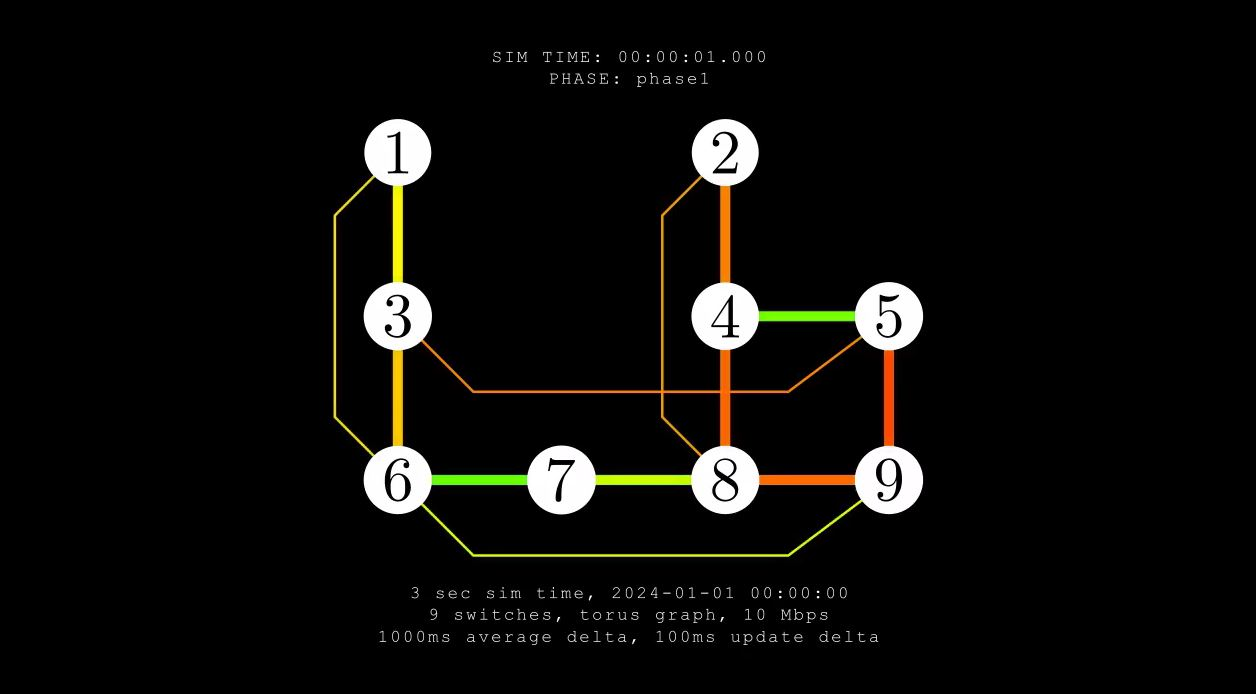
\includegraphics[width=0.8\textwidth]{immagini/only_links.JPG}
    \caption{a nice plot}
    \label{fig:only_links}
\end{figure}

As you can see in the figure \ref{fig:only_links}, the 
function grows near 0. Also, in the page \pageref{fig:only_links} 
is the same example.


\printbibliography

\backmatter
\cleardoublepage
\phantomsection % Give this command only if hyperref is loaded
\addcontentsline{toc}{chapter}{\bibname}
% Here put the code for the bibliography. You can use BibTeX or
% the BibLaTeX package or the simple environment thebibliography.
\end{document}